\documentclass[
    12pt,
    openright,
    oneside,
    a4paper
]{abntex2}

% ---
% Pacotes básicos
% ---
\usepackage{lmodern}
\usepackage[T1]{fontenc}
\usepackage[utf8]{inputenc}
\usepackage[brazil]{babel}
\usepackage{indentfirst}
\usepackage{color}
\usepackage{graphicx}
\usepackage{microtype}
\usepackage{amsmath, amssymb, amsfonts}
\usepackage{geometry}
\usepackage{setspace}
\usepackage{booktabs}
\usepackage{longtable}
\usepackage{array}
\usepackage{enumitem}
\usepackage{csquotes}
\usepackage{float}
\usepackage{hyperref}

% ---
% Configurações do pacote hyperref
% ---
\hypersetup{
    colorlinks=true,
    linkcolor=blue,
    citecolor=blue,
    filecolor=blue,
    urlcolor=blue,
    pdftitle={Relatório de Testes de Usabilidade - PetCuida Alpha 3i},
    pdfauthor={Gabriel da Silva Cassino, Giovanna Naves Ribeiro, Júlia Rodrigues Vasconcellos Melo, Kathleen Rodrigues Leite Barbosa},
    pdfsubject={Atividade 6 - Tópicos III - Empreendedorismo e Inovação},
    pdfkeywords={usabilidade, teste de usuário, PetCuida, satisfação, protótipo},
}

% ---
% Margens e espaçamento (ABNT NBR 14724:2011)
% ---
\geometry{left=3cm, right=2cm, top=3cm, bottom=2cm}
\OnehalfSpacing

% ---
% Ambiente para turnos de fala reaproveitado das entrevistas formalizadas
% ---
\newenvironment{turnos}
  {\begin{list}{}{%
     \setlength{\leftmargin}{2.2cm}%
     \setlength{\labelwidth}{2.0cm}%
     \setlength{\labelsep}{0.2cm}%
     \setlength{\itemsep}{0.45em}%
     \setlength{\parsep}{0pt}}}
  {\end{list}}
\newcommand{\fala}[1]{\item[\textbf{#1}\hfill]}

\begin{document}

% =============================================================
% Capa
% =============================================================
\begin{capa}
    \begin{center}
        
\includegraphics[width=0.3\textwidth]{./images/brasao.png}

        \vspace*{0.5cm}

        {\Large \textbf{PONTIFÍCIA UNIVERSIDADE CATÓLICA DE MINAS GERAIS}}

        \vspace{0.25cm}
        {\large Campus Coração Eucarístico}

        \vspace{0.25cm}
        {\large Curso: Engenharia de Computação}

        \vspace{0.25cm}
        {\large Disciplina: Tópicos III - Empreendedorismo e Inovação}

        \vfill

        {\Huge \textbf{Relatório de Testes de Usabilidade}}

        \vspace{0.25cm}
        {\Large Aplicativo PetCuida - versão \textit{Alpha 3i}}

        \vspace{0.25cm}
        {\large (Atividade 6 - Grupo 4)}

        \vfill

        {\Large \textbf{Alunos:}} \\
        \large Gabriel da Silva Cassino \\
        \large Giovanna Naves Ribeiro \\
        \large Júlia Rodrigues Vasconcellos Melo \\
        \large Kathleen Rodrigues Leite Barbosa

        \vspace{0.5cm}

        {\Large \textbf{Professor-Orientador:}} \\
        \large João Carlos Oliveira Caetano

        \vspace{0.25cm}

        {\Large \textbf{Professor-Tutor:}} \\
        \large Paulo Mattos

        \vfill

        {\large \textbf{Belo Horizonte}}\\
        {\large \textbf{\the\year}}

    \end{center}
\end{capa}

% =============================================================
% Folha de rosto
% =============================================================
\begin{folhaderosto}
    \begin{center}

        {\large \textbf{Gabriel da Silva Cassino}} \\
        {\large \textbf{Giovanna Naves Ribeiro}} \\
        {\large \textbf{Júlia Rodrigues Vasconcellos Melo}} \\
        {\large \textbf{Kathleen Rodrigues Leite Barbosa}}

        \vfill

        {\Large \textbf{Relatório de Testes de Usabilidade}}

        \vspace{0.25cm}
        {\Large Aplicativo PetCuida - versão \textit{Alpha 3i}}

        \vfill

    \end{center}

    \begin{flushright}
        \begin{minipage}{8cm}
            \SingleSpacing
                {\small
                Trabalho acadêmico apresentado à disciplina
                Tópicos III - Empreendedorismo e Inovação,
                do Curso de Engenharia de Computação da
                Pontifícia Universidade Católica de Minas
                Gerais, como requisito parcial para obtenção
                de nota, referente à Atividade 6 - Relatório
                de testes de usabilidade.
                }

                \vspace{0.5cm}
                {\small
                \textbf{Professor-Orientador:} \\Prof. João Carlos Oliveira Caetano \\
                \textbf{Professor-Tutor:} \\Prof. Paulo Mattos
                }
            \OnehalfSpacing
        \end{minipage}
    \end{flushright}

    \vfill

    \begin{center}
        {\large \textbf{Belo Horizonte}} \\
        {\large \textbf{\the\year}}
    \end{center}

\end{folhaderosto}

\tableofcontents
\listoffigures
\listoftables
\newpage

% =============================================================
\chapter{Introdução}

Este relatório documenta o planejamento, a execução e a análise dos \textbf{testes de
usabilidade} conduzidos pelo Grupo 4 sobre o protótipo funcional do aplicativo
\textbf{PetCuida}, em sua versão \textit{Alpha 3i}, conforme orientação da disciplina Tópicos
III - Empreendedorismo e Inovação (Atividade 6). O objetivo geral é avaliar a experiência do
usuário, a facilidade de uso e a efetividade das funcionalidades da solução proposta, acerca
dos blocos de proposta de valor e segmentação de clientes definidos em etapas anteriores do
projeto.

O PetCuida propõe intermediar, em uma única plataforma, tutores que precisam de serviços de
cuidado animal e pessoas ou profissionais dispostos a ofertá-los, um modelo descrito pelo
próprio grupo como \enquote{Uber \textit{Pet} de mão dupla}, remunerado por meio de
créditos internos ou de valores reduzidos (\enquote{preço social}), além de triagem
orientativa, prontuário do animal, calendário de vacinas e uma rede solidária com clínicas
parceiras.

Os testes reunidos neste relatório abrangem cinco sessões com participantes de perfis
complementares. As duas primeiras foram conduzidas por Gabriel com moradoras de um mesmo
bairro de Sabará, a sra.~Aline e, em sessão separada, as senhoras Galdina e
Atanizia, representando o segmento primário de tutores de classes C, D e E com barreiras
econômicas de acesso a cuidados veterinários. As demais foram conduzidas separadamente por
Kathleen, Júlia e Giovanna: a pessoa entrevistada por Kathleen foi Calebe Henrique, de
16~anos, morador da Região Metropolitana de Belo Horizonte e tutor de um cachorro; a
pessoa entrevistada por Júlia foi o sr.~Lucas; e a pessoa entrevistada por Giovanna foi a
sra.~Flávia, tutora de pet de pequeno porte e pertencente à classe média alta. Há entrevistas
formalizadas para as Sessões~1, 2, 3 e~5, enquanto a Sessão~4 foi registrada por meio de
anotações dos pontos mais relevantes. Essa combinação permite cruzar percepções de
participantes de diferentes contextos acerca do aplicativo.

\section{Evidências e repositório do projeto}

O código-fonte do protótipo Flutter avaliado, o histórico de desenvolvimento e os materiais
completos de suporte a este relatório, incluindo as entrevistas formalizadas na íntegra e
as transcrições em \texttt{.txt}/\texttt{.srt}, estão disponíveis no repositório do projeto:

\begin{center}
\url{https://github.com/kasshinokun/Q3_Q4_2026_Public/tree/main/TOPICOS_III/Atividade_VI}
\end{center}

\textit{- Os áudios foram transcritos com IA, porém corrigidos e adaptados para semiliteral pelos alunos, objetivando o entendimento dos leitores deste documento} 

\newpage
Um registro em vídeo com evidências da execução dos testes de usabilidade descritos neste
documento está disponível em:

\begin{center}
\url{https://youtu.be/uS83wGpVHdg}
\end{center}

% =============================================================
\chapter{Planejamento do Teste}

\section{Objetivos do teste}

Definiram-se os seguintes objetivos para as sessões de teste:

\begin{enumerate}[label=\textbf{O\arabic*.}, leftmargin=1.6cm]
  \item Verificar se as pessoas participantes conseguem compreender, sem apoio técnico prévio, a
        proposta funcional do PetCuida ao serem apresentadas ao protótipo.
  \item Observar se os elementos de interface (autenticação, cadastro do pet, área do pet,
        triagem, rede solidária e perfil) são interpretados corretamente quanto à sua função.
  \item Registrar a percepção qualitativa de facilidade de uso e de utilidade, incluindo
        eventuais dificuldades, confusões ou pontos de destaque durante a navegação.
  \item Verificar a aderência das funcionalidades demonstradas à proposta de valor do
        projeto (intermediação de serviços, sistema de créditos, triagem orientativa e rede
        solidária) e ao segmento de clientes previamente definido.
  \item Coletar sugestões de melhoria que possam orientar as próximas revisões do protótipo.
\end{enumerate}

\newpage
\section{Participantes e segmentos representados}

A Tabela~\ref{tab:participantes} relaciona as sessões realizadas, a pessoa entrevistada em
cada uma delas e o segmento de cliente que ela melhor representa dentro da proposta do
projeto.

\begin{table}[H]
\centering
\small
\begin{tabular}{@{}>{\raggedright\arraybackslash}p{2.6cm}>{\raggedright\arraybackslash}p{4.4cm}>{\raggedright\arraybackslash}p{6.3cm}@{}}
\toprule
\textbf{Sessão} & \textbf{Entrevistador(a) / participante} & \textbf{Segmento representado} \\
\midrule
1 & Entrevistador: Gabriel. Participante: Sra.~Aline. & Tutora individual, usuária leiga em
tecnologia, primeiro contato com o conceito do aplicativo. \\
\addlinespace
2 & Entrevistador: Gabriel. Participantes: Sra.~Galdina e Sra.~Atanizia. & Moradoras do mesmo
bairro, com relatos de barreiras econômicas e geográficas de acesso a atendimento veterinário
e castração, núcleo do problema que motivou o projeto. \\
\addlinespace
3 & Entrevistadora: Kathleen. Participante: Calebe Henrique, 16 anos, morador da RMBH. &
Adolescente e tutor de um cachorro, representando o perfil de tutor de pet e de usuário jovem
da solução. \\
\addlinespace
4 & Entrevistadora: Júlia. Participante: Sr.~Lucas. & Participante identificado, mas sem dados
demográficos ou perfil de segmento registrados (ver limitações). \\
\addlinespace
5 & Entrevistadora: Giovanna. Participante: Sra.~Flávia. & Tutora de pet de pequeno porte,
pertencente à classe média alta em Belo Horizonte. \\
\bottomrule
\end{tabular}
\caption{Sessões de teste, entrevistadores(as)/participantes e segmentos de cliente
representados.}
\label{tab:participantes}
\end{table}


\section{Roteiro e tarefas propostas}

Para as cinco sessões, por se tratar de participantes sem contato prévio com o protótipo, o
roteiro consistiu em uma \textbf{demonstração guiada}, conduzida pela respectiva
entrevistadora ou entrevistador, seguida de perguntas abertas, cobrindo sequencialmente: tela
de carregamento e login; criação de conta e login simulado via Google; cadastro do pet
(espécie, nome, raça opcional, data de nascimento, foto); painel inicial; área do pet
(vacinação, calendário, prontuário, edição de dados); triagem de serviço; rede solidária
(serviços disponíveis e mapa); e perfil/configurações (termos de uso e política de
privacidade). Ao final, buscou-se registrar: \emph{(i)} a percepção geral do(a) participante
sobre o aplicativo; \emph{(ii)} se o serviço proposto seria interessante para ele(a); e
\emph{(iii)} eventuais sugestões de melhoria.

Na Sessão~4, esse roteiro não foi seguido de forma protocolar e documentada passo a passo
como nas Sessões~1, 2, 3 e~5: Júlia demonstrou o aplicativo ao sr.~Lucas e registrou, por
escrito, apenas os pontos que considerou mais relevantes na fala do participante, sem
preservar a sequência completa da demonstração.

Em nenhuma das cinco sessões a navegação foi executada de
forma autônoma pela pessoa entrevistada, em todas elas, quem manipulou o dispositivo foi
quem conduziu a entrevista. Portanto, não se tratou de teste de usabilidade com execução
autônoma de tarefas, mas de apresentação guiada com coleta de \textit{feedback}. Essa
limitação é retomada na Seção~\ref{sec:limitacoes}.

% =============================================================
\chapter{Execução do Teste}

\section{Sessão 1 - Sra. Aline}

A sessão foi conduzida por Gabriel em formato de demonstração guiada, com duração aproximada
de 7~minutos e 32~segundos de áudio. A participante acompanhou o percurso pelas telas sem
manifestar dificuldade perceptível e comparou espontaneamente a experiência de uso à de um
aplicativo de mensageria de uso cotidiano. A transcrição integral consta no documento \textit{Entrevista\_Formalizada\_Aline}
(Apêndice~\ref{apx:aline}).

\section{Sessão 2 - Sra. Galdina e Sra. Atanizia}

Conduzida também por Gabriel, com as duas participantes presentes na mesma sessão (Atanizia é
mãe do entrevistador), a conversa combinou contextualização do problema social que motivou o
projeto (custo veterinário, abandono, castração e barreiras territoriais) com a
demonstração guiada do protótipo. A sessão teve duração aproximada de 25~minutos e
31~segundos. Ao final, a sra.~Galdina classificou o aplicativo como \enquote{interessante} e
\enquote{fácil}, sem dificuldade aparente na navegação demonstrada, e ambas destacaram a
necessidade de o programa ser mais amplamente divulgado. A transcrição integral consta no
documento \textit{Entrevista\_Galdina\_Atanizia} (Apêndice~\ref{apx:galdina}).

\section{Sessão 3 - Calebe Henrique}

Kathleen demonstrou o protótipo a Calebe Henrique, de 16~anos, morador da Região Metropolitana
de Belo Horizonte e tutor de um cachorro. O participante destacou a triagem orientativa
associada à recomendação de clínica como funcionalidade prática e eficiente, os lembretes de
prazo e a possibilidade de criação de uma comunidade de ajuda. Também sugeriu uma aba
explicativa sobre o funcionamento do sistema de créditos. A transcrição integral consta no
documento \textit{Entrevista\_Formalizada\_Calebe.pdf}
(Apêndice~\ref{apx:calebe}).

\section{Sessão 4 - Sr. Lucas}

Júlia demonstrou o protótipo ao sr.~Lucas e registrou por escrito os pontos que considerou
mais relevantes em sua fala, sem produzir uma transcrição literal e completa. O participante
avaliou a proposta como interessante por reunir diferentes funções relacionadas ao cuidado
animal em um único aplicativo e classificou a navegação como tranquila, com opções
principais fáceis de localizar. O relato consta no Apêndice~\ref{apx:relatos}.

\section{Sessão 5 - Sra. Flávia}

Giovanna conduziu a demonstração do protótipo para a sra.~Flávia. A participante comentou
favoravelmente a área de vacinas, prontuário e calendário, bem como a presença da foto do
tutor. Relatou não compreender bem o funcionamento dos créditos nem a finalidade do QR Code
do pet. 

Além disso, valorizou o suporte humano, as notificações, os lembretes, a triagem de sintomas e o
mapa de clínicas e sugeriu controle de alimentação para pets doentes, um módulo de adoção,
lista de lojas parceiras com promoções e comparação de preços de produtos. A entrevista
formalizada consta no documento \textit{Entrevista\_Formalizada\_Flavia.pdf}
(Apêndice~\ref{apx:flavia}).


\section{Evidências de execução}

As Figuras~\ref{fig:homepage} a~\ref{fig:sobre} ilustram trechos do percurso demonstrado nas
cinco sessões, incluindo a tela inicial, o fluxo de triagem, a rede solidária com serviço de
castração listado, a área do pet com vacinas e prontuário, e
o ajuste de localização do seletor de data para o português, implementado em revisão
posterior à identificação do problema (Seção~\ref{sec:problemas}). O registro em vídeo
referenciado na Seção~1.1 complementa estas evidências estáticas.

\begin{figure}[H]
\centering
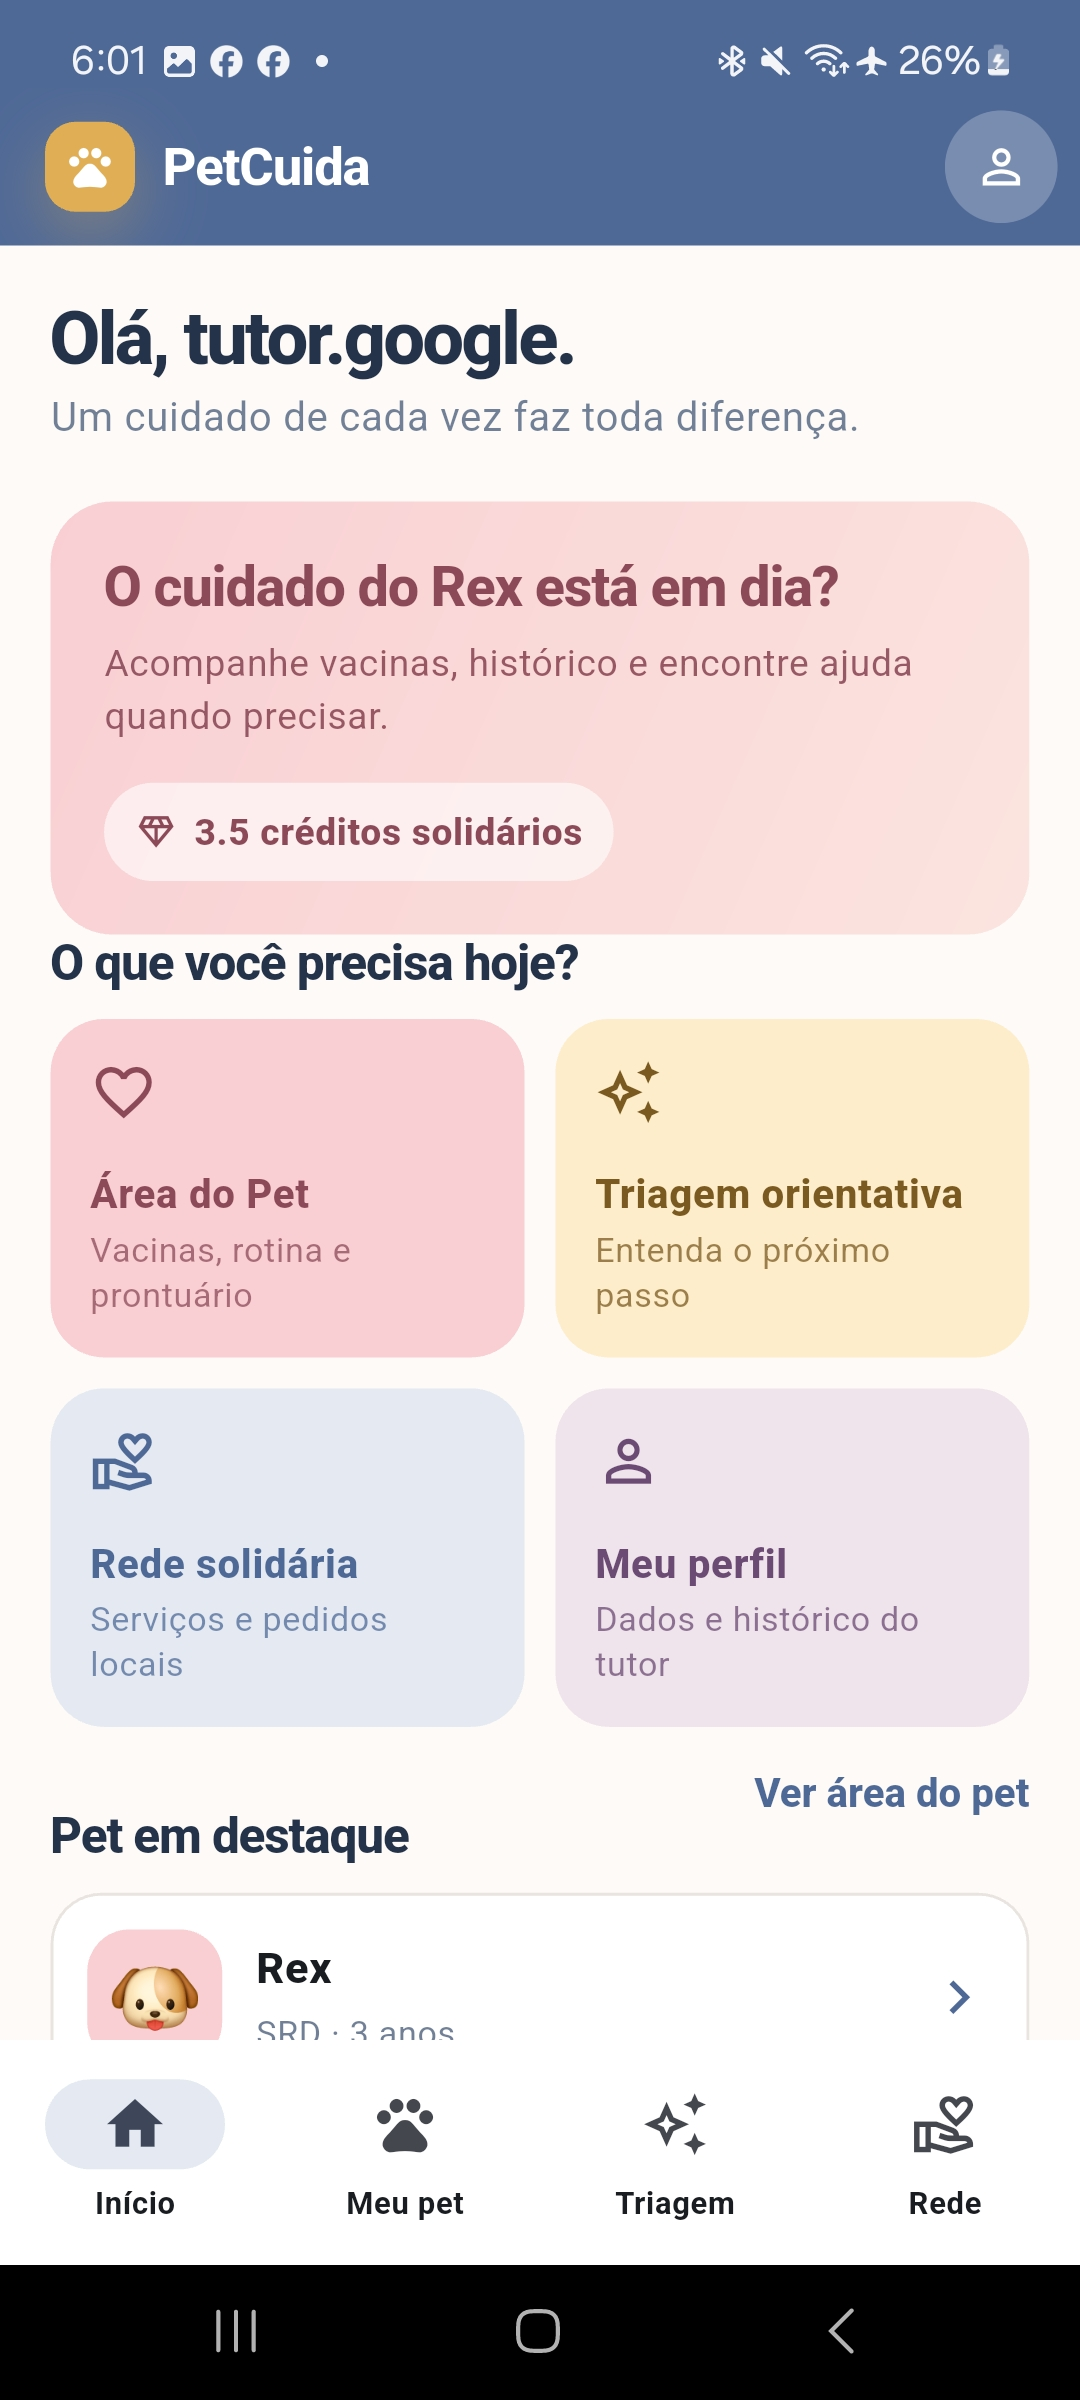
\includegraphics[width=0.42\textwidth]{./images/execucao_v3e/homepage_v3e.jpg}
\caption{Painel inicial do PetCuida, com créditos solidários e acesso às quatro áreas
principais.}
\label{fig:homepage}
\end{figure}

\begin{figure}[H]
\centering
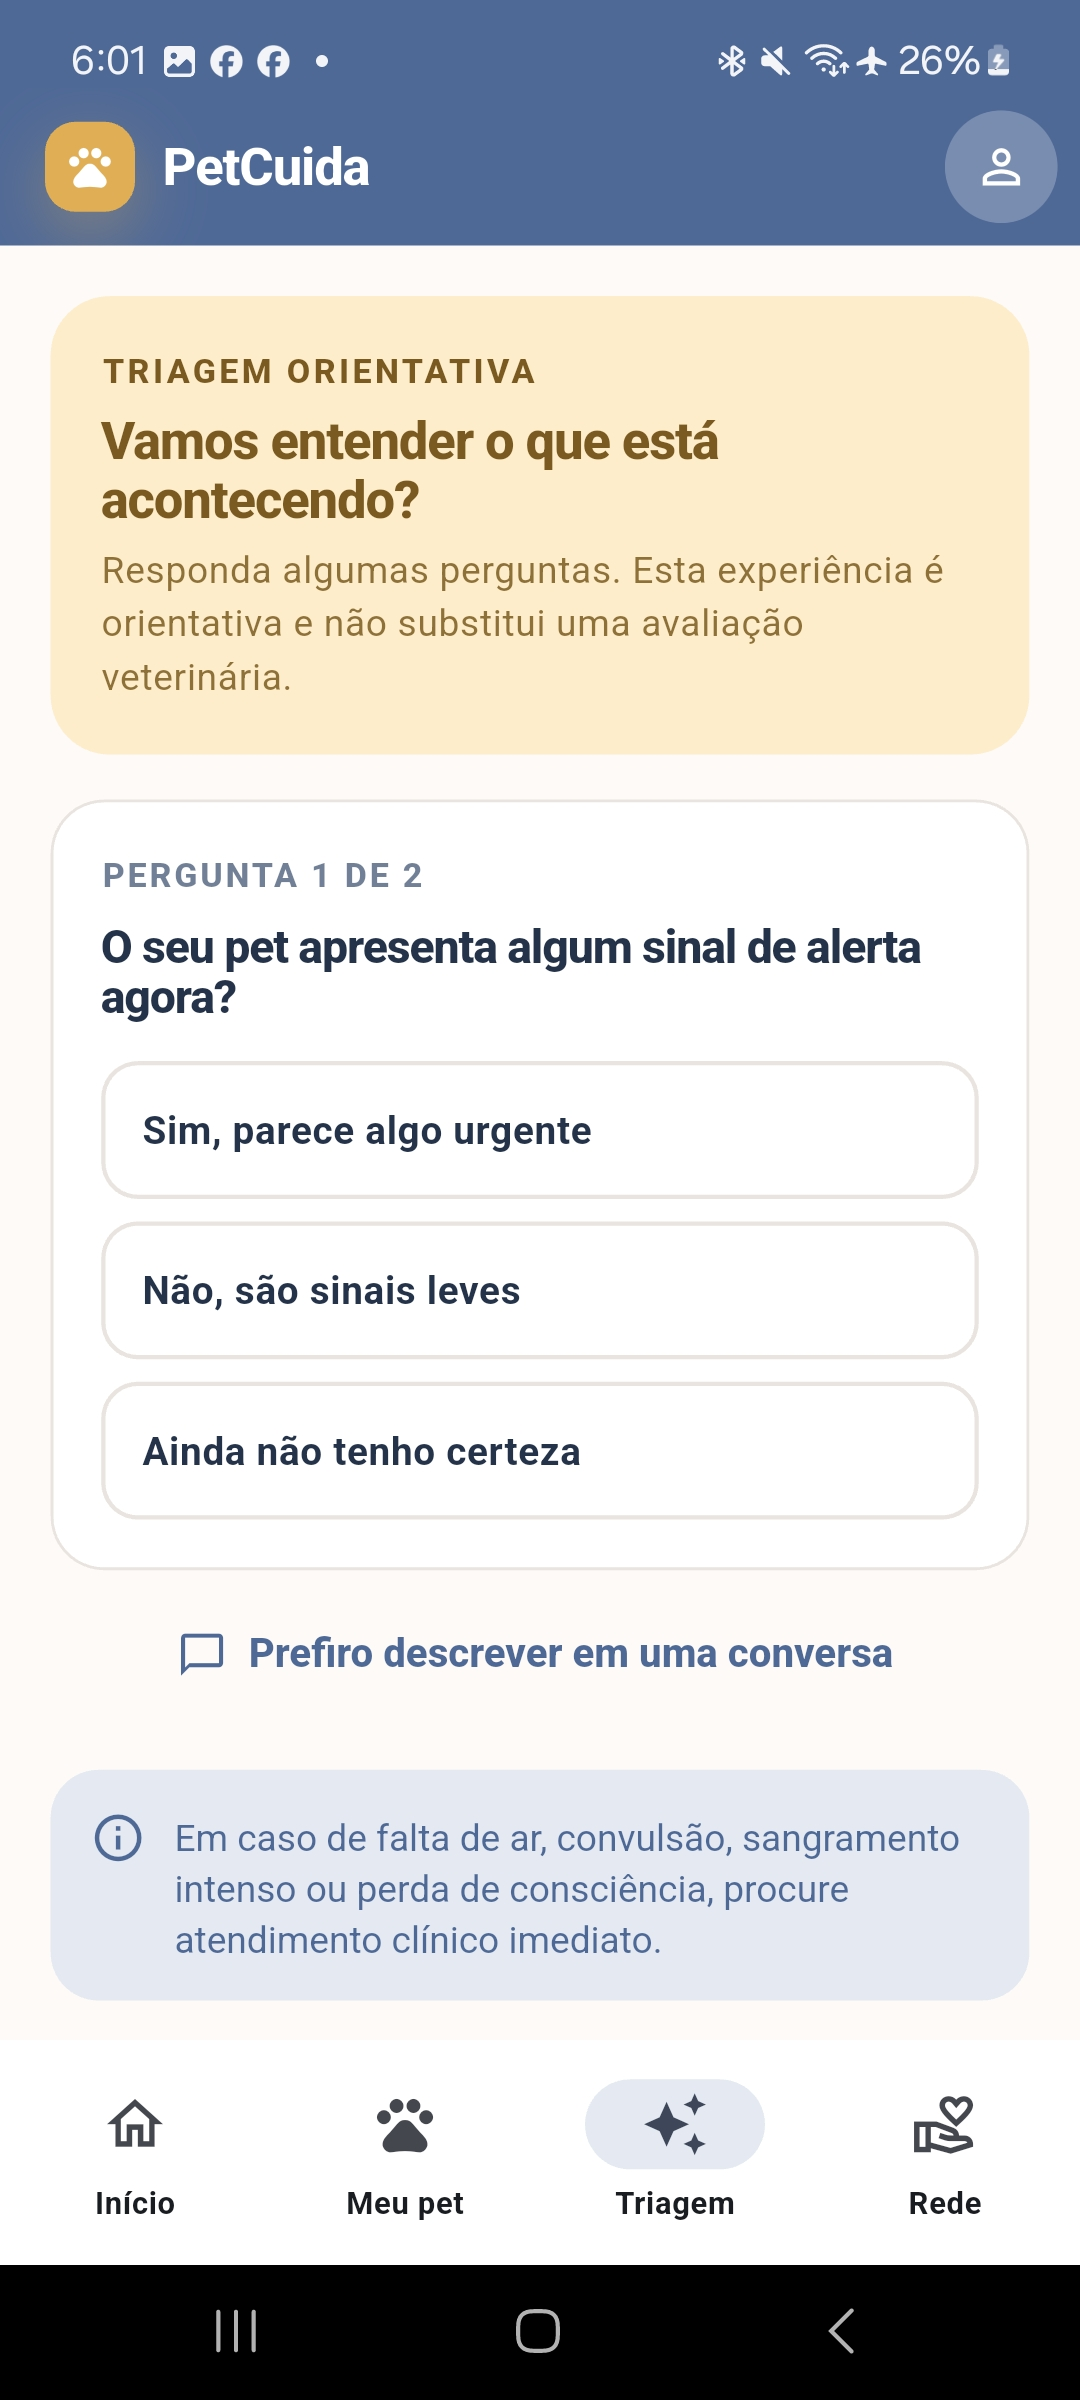
\includegraphics[width=0.42\textwidth]{./images/execucao_v3e/triagem_v3e.jpg}
\caption{Fluxo de triagem orientativa, funcionalidade destacada positivamente por Calebe
Henrique e pela sra.~Flávia.}
\label{fig:triagem}
\end{figure}

\begin{figure}[H]
\centering
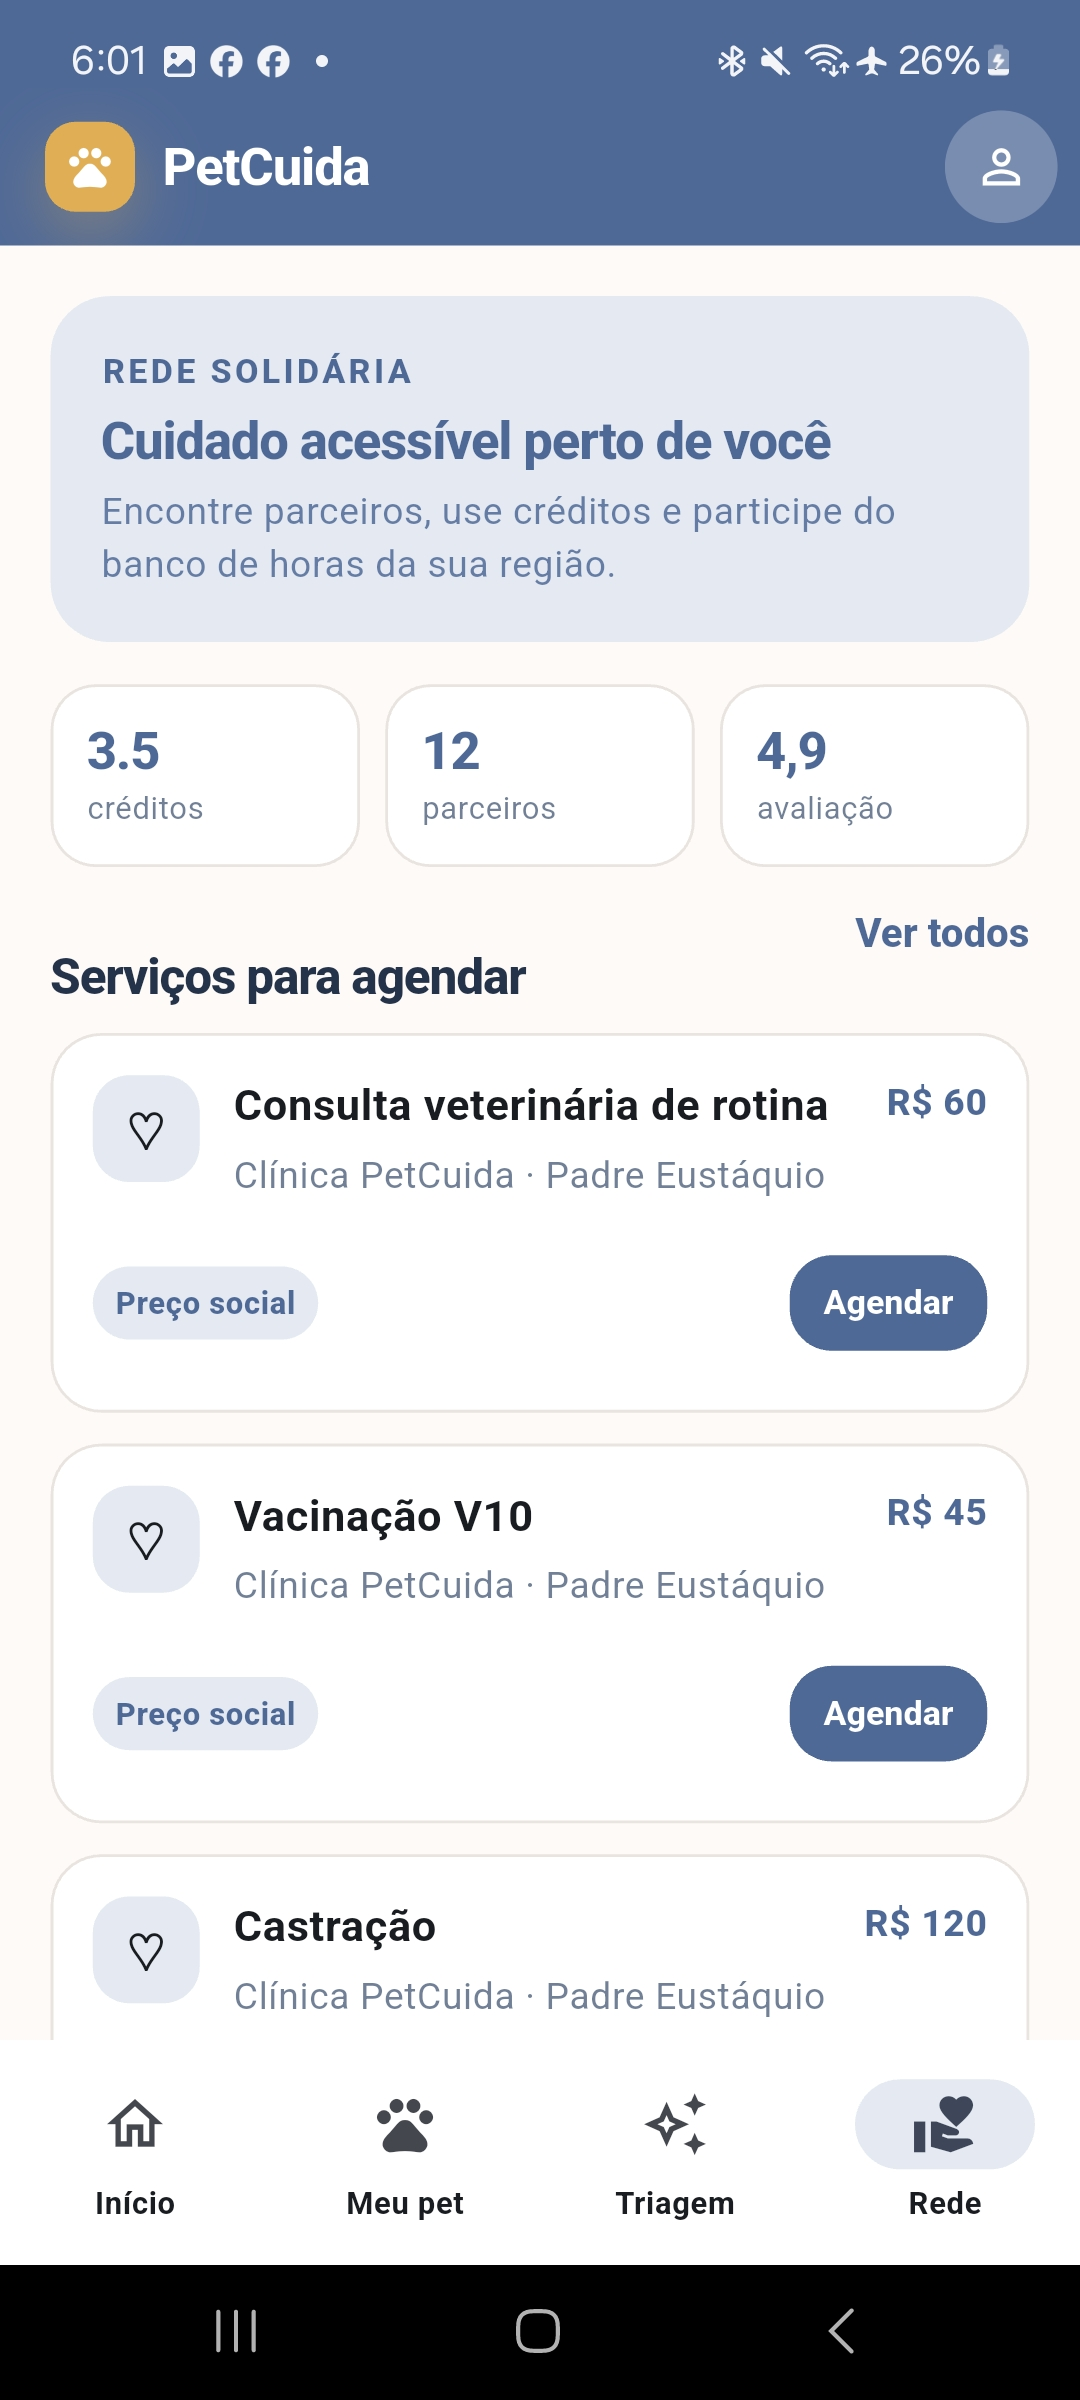
\includegraphics[width=0.42\textwidth]{./images/execucao_v3e/social_network.jpg}
\caption{Rede solidária com serviços de consulta, vacinação e castração a preço social, tema
central da Sessão~2.}
\label{fig:rede}
\end{figure}

\begin{figure}[H]
\centering
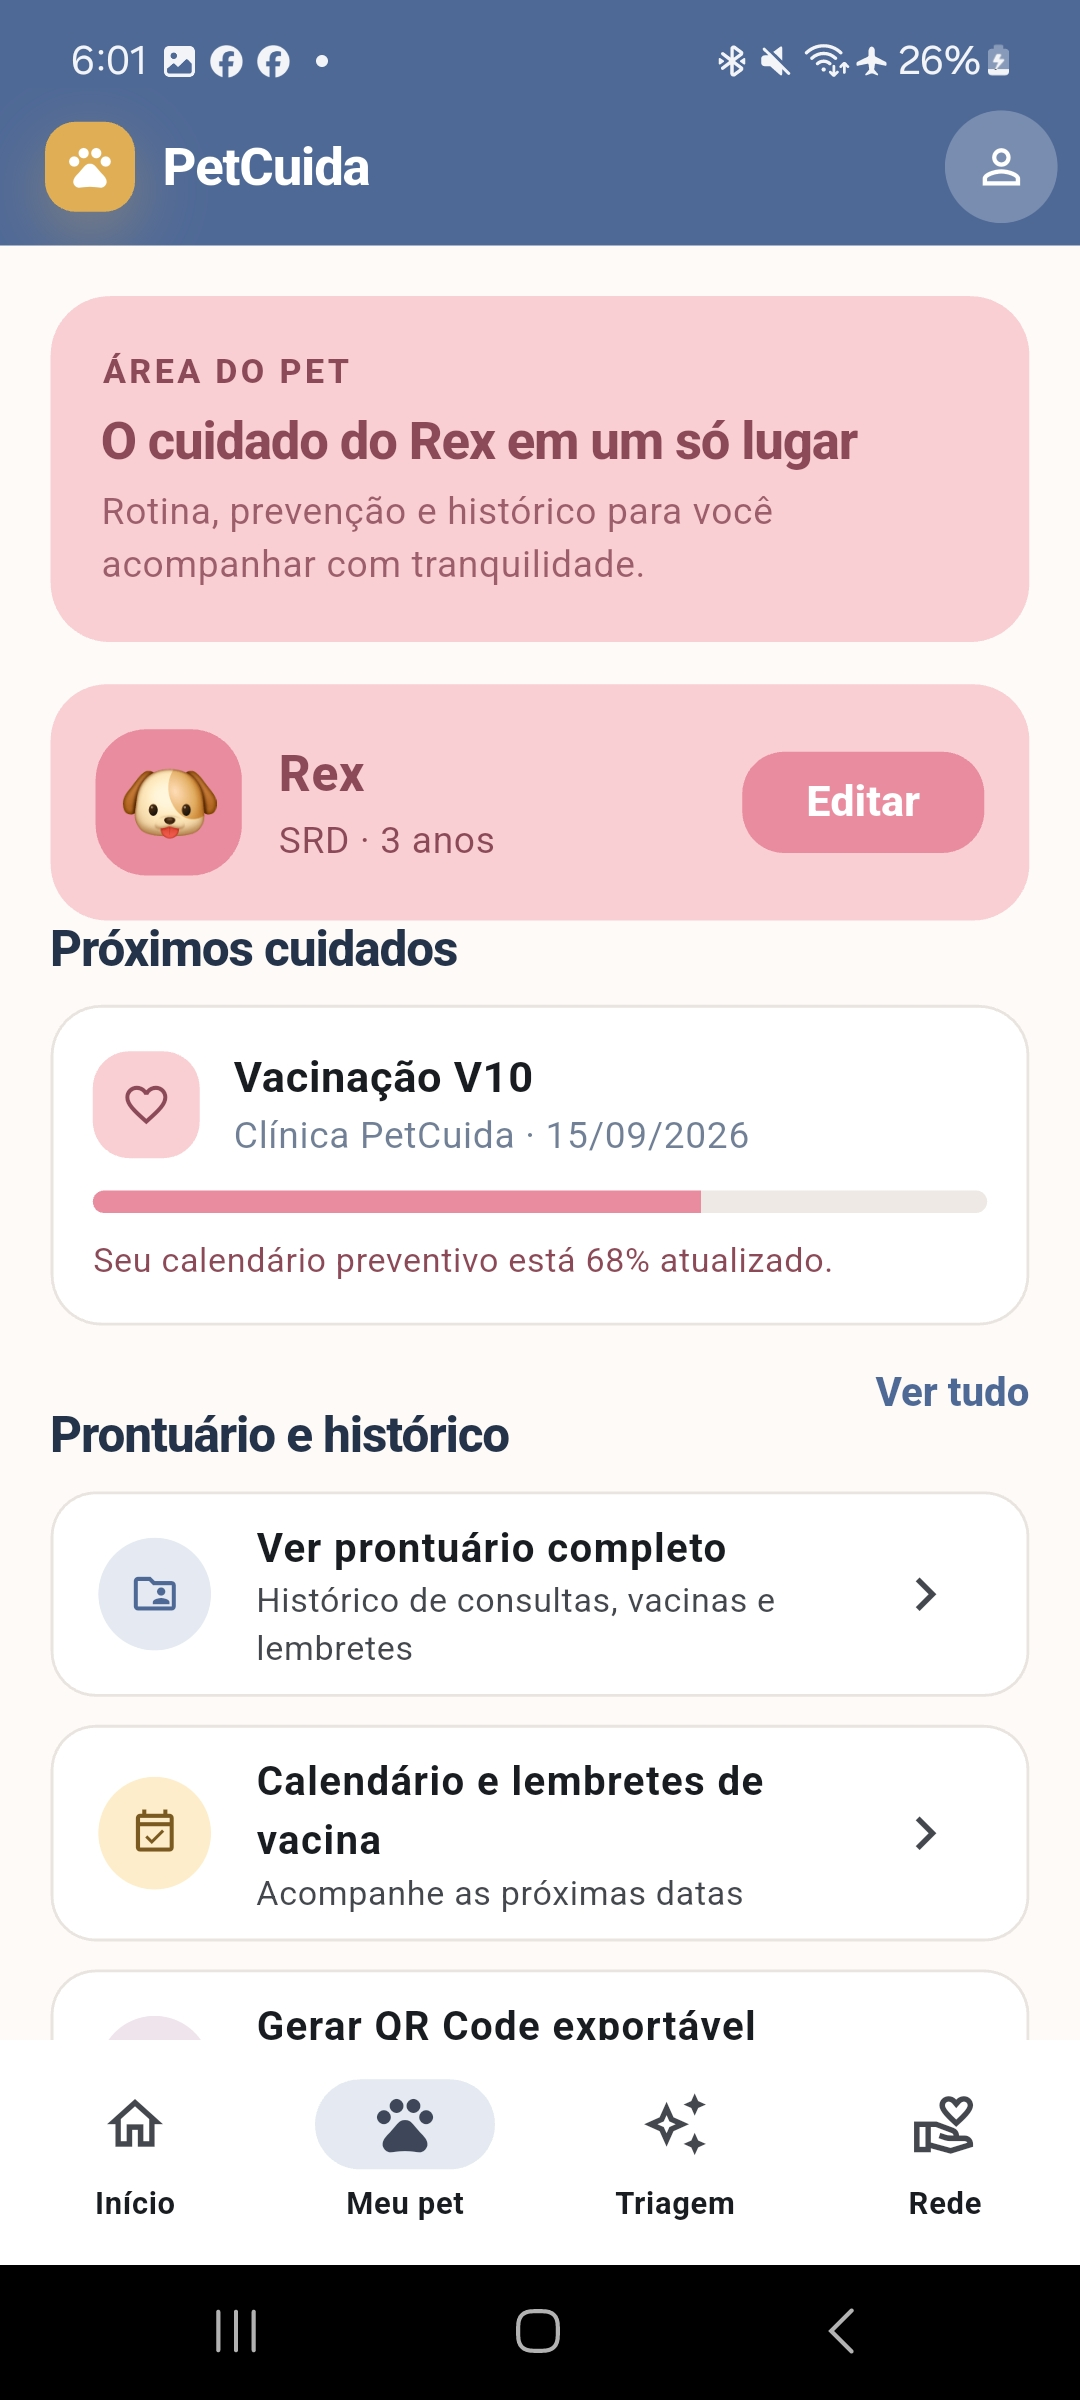
\includegraphics[width=0.42\textwidth]{./images/execucao_v3e/pet_profile_v3e.jpg}
\caption{Área do pet, com calendário preventivo, prontuário e geração de QR Code.}
\label{fig:petprofile}
\end{figure}

\begin{figure}[H]
\centering
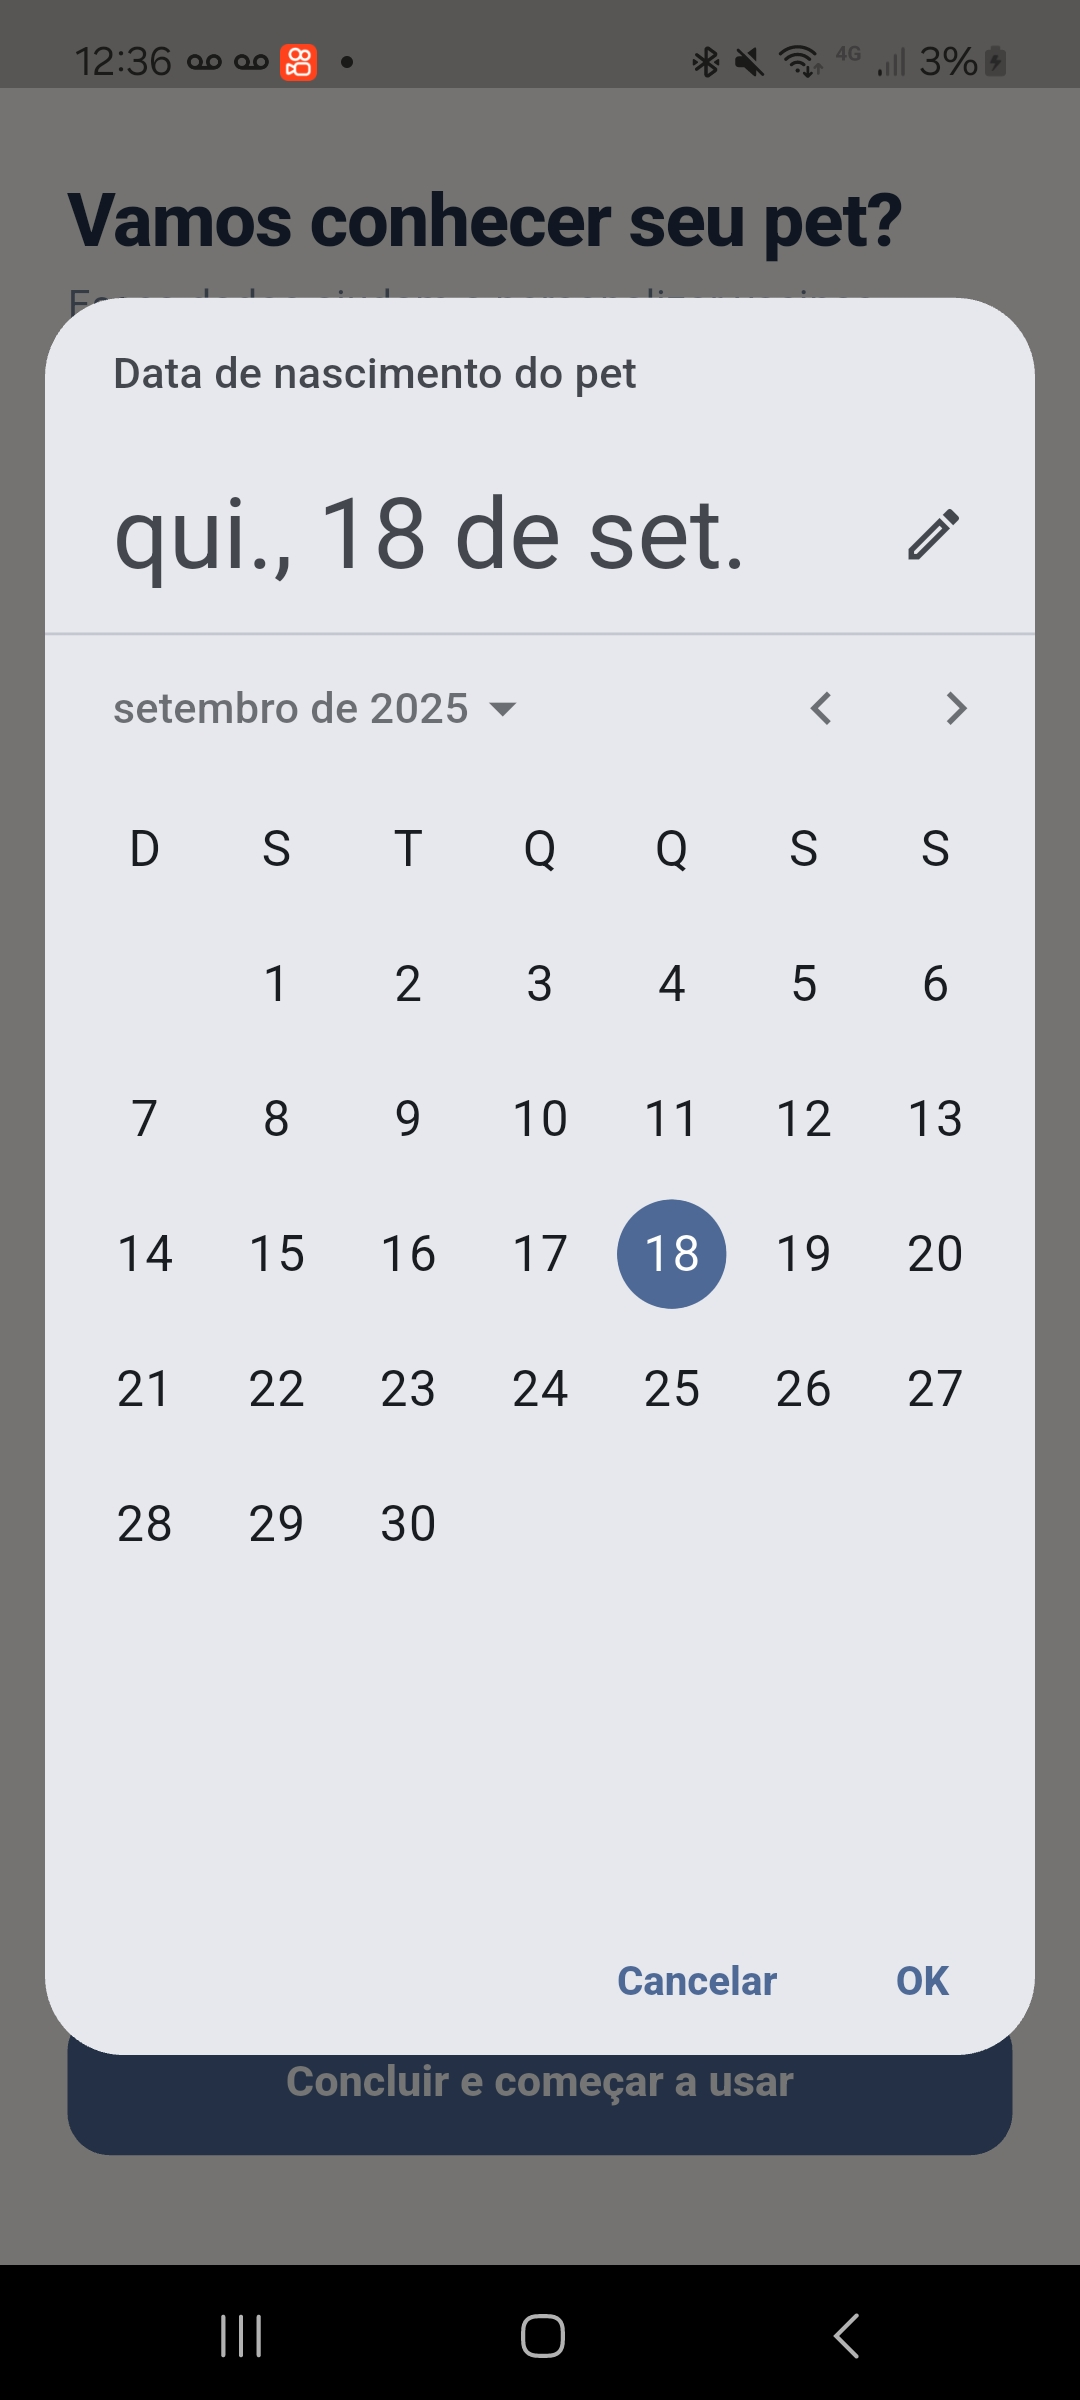
\includegraphics[width=0.42\textwidth]{./images/execucao_3i2k/calendar_as_br.jpg}
\caption{Seletor de data localizado em português, corrigindo a limitação relatada em padrão
americano durante as Sessões 1 e 2.}
\label{fig:calendario}
\end{figure}

\begin{figure}[H]
\centering
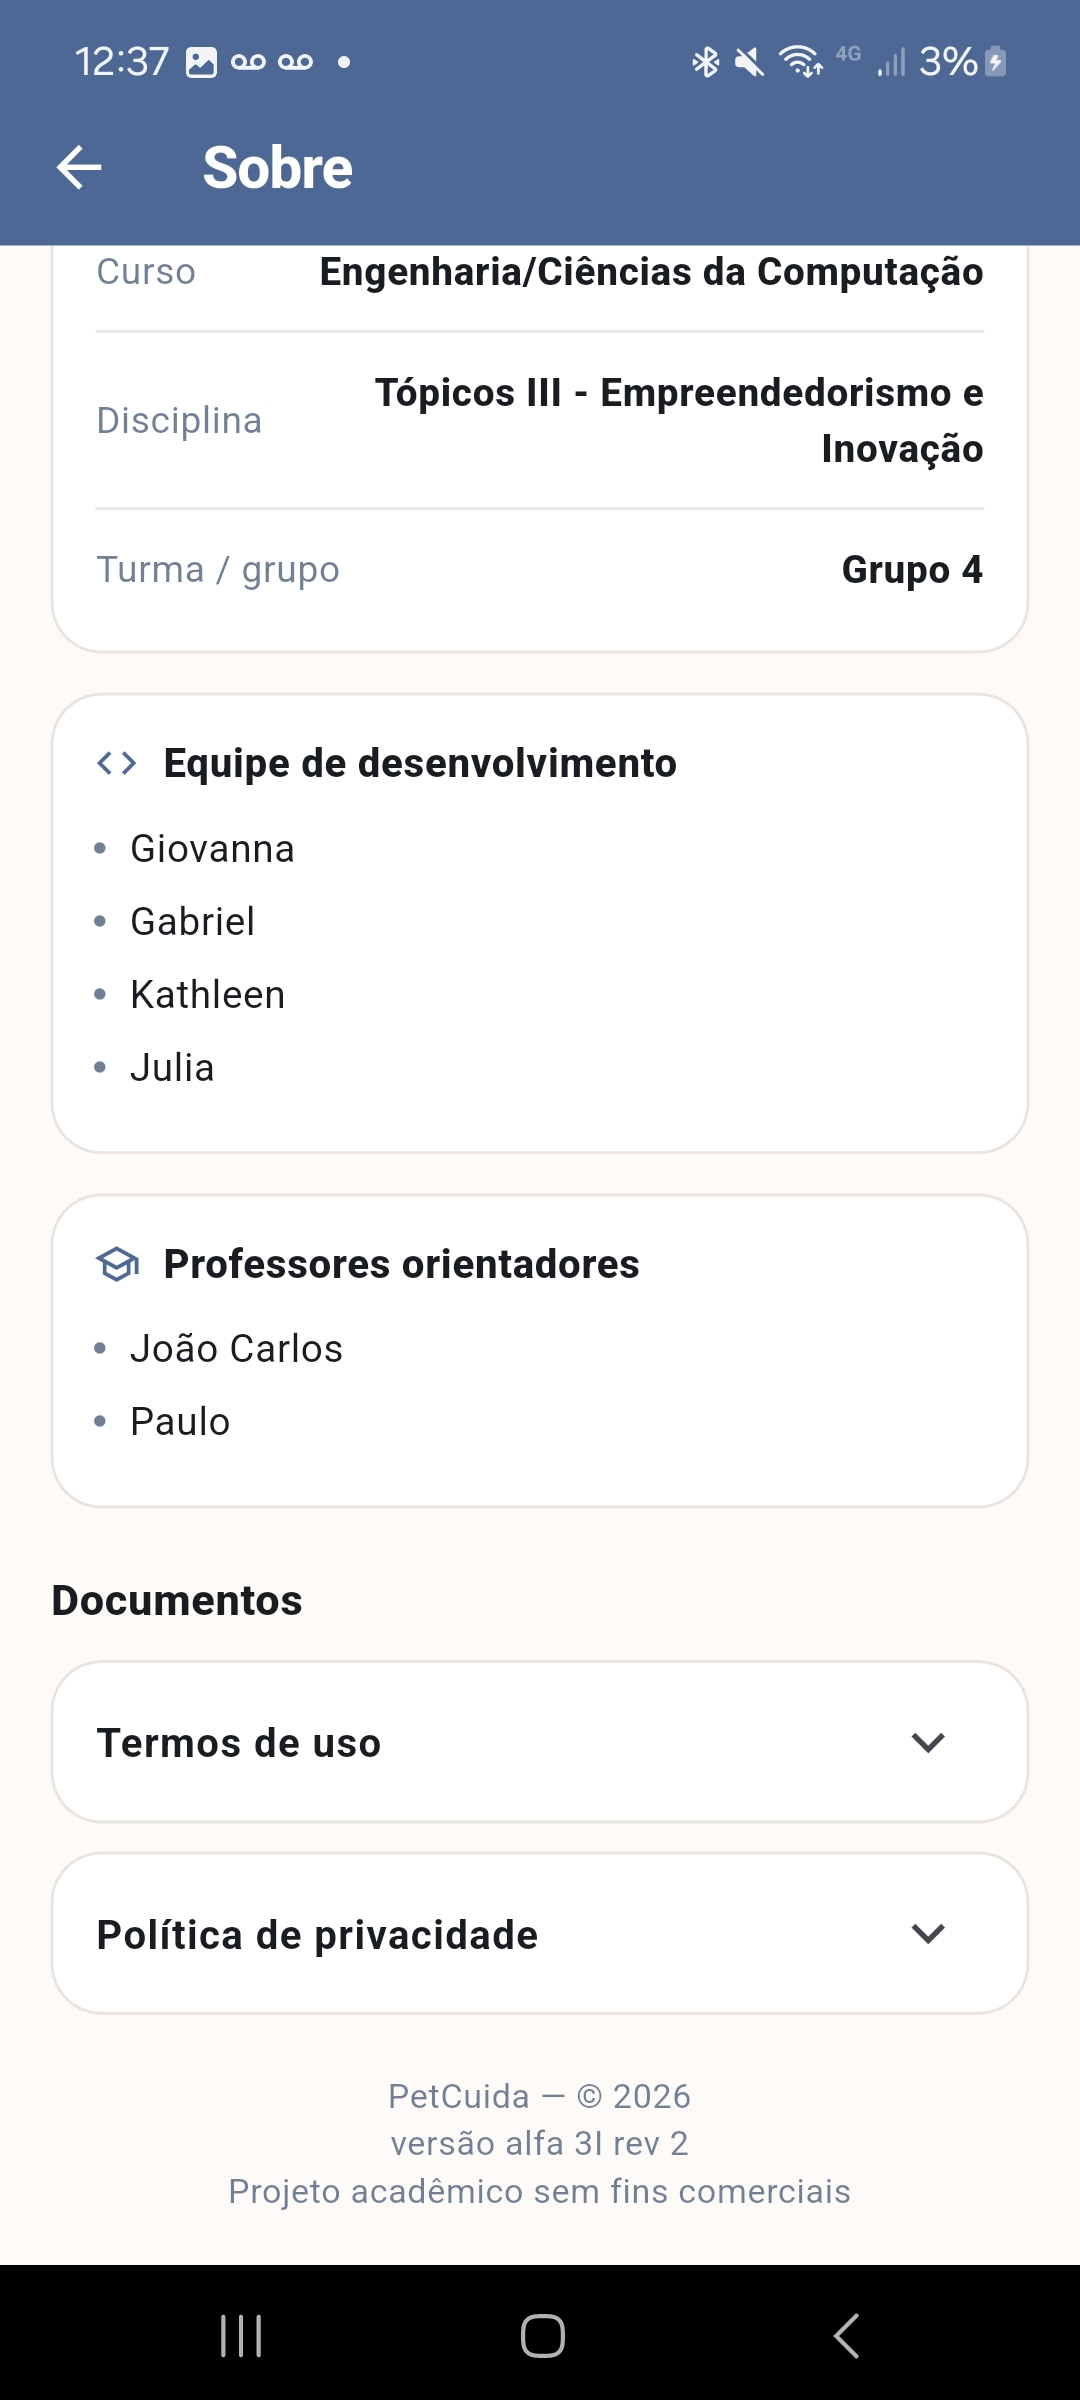
\includegraphics[width=0.42\textwidth]{./images/execucao_3i2k/versao_as_var.jpg}
\caption{Tela \enquote{Sobre} do protótipo, identificando equipe, orientadores e versão
avaliada (alfa 3i, rev.~2).}
\label{fig:sobre}
\end{figure}

% =============================================================
\chapter{Documentação e Análise}

\section{Problemas encontrados}
\label{sec:problemas}

\begin{table}[H]
\centering
\small
\begin{tabular}{@{}>{\raggedright\arraybackslash}p{4.3cm}>{\raggedright\arraybackslash}p{4.3cm}>{\raggedright\arraybackslash}p{5.3cm}@{}}
\toprule
\textbf{Problema observado} & \textbf{Origem} & \textbf{Situação} \\
\midrule
Seletor de data em formato norte-americano, não localizado & Sessões 1 e 2 (relato do
entrevistador durante a demonstração) & Corrigido na revisão \textit{rev.~2}, com exibição em
português (Figura~\ref{fig:calendario}) \\
\addlinespace
Login por conta Google apenas simulado, sem integração real & Sessões 1 e 2 & Limitação
conhecida do estágio alfa, documentada no repositório do projeto \\
\addlinespace
Finalidade do QR Code do prontuário não compreendida pela participante & Sessão~5
(Sra.~Flávia) & Em aberto, recomenda-se texto explicativo na própria tela \\
\addlinespace
Funcionamento do sistema de créditos pouco claro & Sessão~3 (Calebe Henrique) e Sessão~5
(Sra.~Flávia) & Em aberto, recomenda-se aba ou tutorial inicial
explicando o sistema de créditos \\
\addlinespace
Mapa da rede solidária esquemático, sem georreferenciamento real & Sessões 1 e 2 & Limitação
conhecida do estágio alfa \\
\addlinespace
Navegação conduzida por quem entrevistava, sem execução autônoma de tarefas pela pessoa
participante & Todas as sessões (1 a 5) & Limitação do protocolo de teste, não do protótipo
(Seção~\ref{sec:limitacoes}) \\
\bottomrule
\end{tabular}
\caption{Problemas identificados nas sessões de teste, origem e situação atual.}
\label{tab:problemas}
\end{table}

\section{Aspectos positivos}

\begin{itemize}[leftmargin=*]
  \item \textbf{Facilidade de uso percebida.} Aline e Galdina relataram facilidade de uso sem
        dificuldade aparente, com Aline comparando a experiência a um aplicativo de
        mensageria já dominado.
  \item \textbf{Clareza da triagem orientativa.} Apontada por Calebe Henrique como
        prática e eficiente por recomendar diretamente uma clínica a partir de uma breve
        descrição do problema do pet, e pela sra.~Flávia como útil para
        compreender o problema antes de buscar atendimento.
  \item \textbf{Unificação de funcionalidades.} No relato do sr.~Lucas, destacou-se como
        diferencial reunir, em um único aplicativo, funções normalmente dispersas em soluções
        distintas.
  \item \textbf{Interface visual.} O sr.~Lucas qualificou a interface como bonita, com
        navegação tranquila e opções principais fáceis de localizar.
  \item \textbf{Aderência ao problema social identificado.} Na Sessão~2, o serviço de
        castração a preço social e a intermediação de transporte e atendimento foram
        reconhecidos por Galdina e Atanizia como resposta direta a barreiras já vividas na
        comunidade (custo, distância e concentração de atendimento em Belo Horizonte).
  \item \textbf{Suporte, lembretes e notificações.} A sra.~Flávia e Calebe Henrique
        destacaram positivamente os lembretes de
        calendário/vacinação; a sra.~Flávia também valorizou a existência de suporte humano
        dentro do aplicativo.
\end{itemize}

\section{Sugestões de melhoria}

\begin{enumerate}[label=\textbf{S\arabic*.}, leftmargin=1.6cm]
  \item Incluir uma seção explicativa (\textit{tutorial} ou aba dedicada) sobre o
        funcionamento do sistema de créditos, incluindo como são gerados e utilizados
        (Sessões~3 e~5).
  \item Explicitar, na própria tela, a finalidade do QR Code do prontuário do pet
        (sugestão da sra.~Flávia).
  \item Adicionar controle de alimentação para pets em tratamento ou doentes (sugestão da
        sra.~Flávia).
  \item Incluir módulo de adoção de animais dentro da plataforma (sugestão da
        sra.~Flávia).
  \item Adicionar lista de lojas parceiras de produtos pet, com promoções e comparação de
        preços entre estabelecimentos (sugestão da sra.~Flávia).
  \item Ampliar a divulgação do aplicativo junto à comunidade, citada como condição para que
        o serviço proposto seja efetivamente utilizado (Galdina).
  \item Confirmar a georreferenciação real do mapa da rede solidária e a integração efetiva
        do login por conta Google em versões futuras (limitações já conhecidas do estágio
        alfa).
\end{enumerate}

\section{Relação com os objetivos do teste e a proposta de valor}

Os resultados atendem aos objetivos O1 a O5 definidos na Seção~2.1 com ressalvas. Quanto à
\textbf{compreensão da proposta} (O1), as pessoas participantes das cinco sessões demonstraram
entender corretamente o modelo de intermediação de mão dupla, ainda
que os participantes das Sessões~3 e~5 não tenham compreendido plenamente o sistema de créditos (e na Sessão~5, também foi levantada uma limitação no entendimento da função do QR Code). Quanto à
\textbf{interpretação dos elementos de interface} (O2), a triagem, a área do pet e a rede
solidária foram corretamente identificadas em função e propósito em todas as sessões; o
sistema de créditos foi o elemento cuja função gerou dúvida mais recorrente. Quanto à
\textbf{facilidade e utilidade percebidas} (O3), a avaliação foi majoritariamente positiva em
todas as sessões, sem relatos de frustração ou abandono de tarefa.

Quanto à \textbf{aderência à proposta de valor e ao segmento de clientes} (O4), as barreiras relatadas por Galdina e Atanizia na Seção 2, como custo de consulta,
transporte inadequado, concentração de atendimento em Belo Horizonte e dificuldade de acesso
à castração, correspondem exatamente aos serviços listados na rede solidária demonstrada
(Figura~\ref{fig:rede}), o que sustenta a pertinência da proposta de valor para o segmento de
tutores de baixa renda. A Sessão~3 acrescenta a percepção de Calebe Henrique, tutor de um
cachorro, com 16~anos e residente na RMBH, enquanto a Sessão~5 representa a percepção da
sra.~Flávia, tutora de pet de pequeno porte e pertencente à classe média alta. Esses dois
perfis confirmam o interesse de tutores de diferentes faixas etárias e condições
socioeconômicas. Por fim, quanto à \textbf{coleta de sugestões} (O5), as sessões produziram
recomendações concretas e acionáveis, listadas na Seção~4.3, que podem orientar o
\textit{backlog} da próxima revisão do protótipo.

% =============================================================
\chapter{Limitações do Processo de Teste}
\label{sec:limitacoes}

\begin{enumerate}[leftmargin=*]
  \item \textbf{Ausência de execução autônoma de tarefas em todas as sessões.} Em nenhuma das
        cinco sessões a pessoa entrevistada manipulou o dispositivo de forma independente. Em todas, quem conduziu a navegação foi quem entrevistava. Isso impede medir taxa de
        sucesso, tempo de tarefa ou número de erros de forma objetiva.
  \item \textbf{Identificação e perfil dos participantes.} Para o sr.~Lucas, participante da Sessão~4, não
        foram registrados dados demográficos suficientes para relacioná-lo com precisão a um
        segmento de cliente. Além disso, o registro da Sessão~4 consiste apenas nos pontos
        que Júlia considerou mais relevantes, e não em transcrição literal e completa como
        as disponíveis para as Sessões~1, 2, 3 e~5.
  \item \textbf{Amostra pequena e não representativa estatisticamente.} Cinco sessões com
        participantes de perfis distintos permitem apenas leitura exploratória e
        qualitativa.
  \item \textbf{Proximidade entre quem entrevistou e quem foi entrevistado, quando
        identificável.} Atanizia é mãe do entrevistador Gabriel, e Aline e Galdina são
        moradoras próximas com relação prévia a ele, o que favorece potencial viés de
        cortesia nas respostas. A sra.~Flávia é mãe da entrevistadora Giovanna, de modo que
        esse mesmo risco também se aplica à Sessão~5. Para as Sessões~3 e~4, a relação entre
        cada aluna e o respectivo participante não foi informada, não sendo possível avaliar
        esse risco.
  \item \textbf{Ausência de instrumento padronizado de usabilidade.} Não foi aplicada escala
        validada (como a \textit{System Usability Scale} - SUS), o que impede comparação
        numérica entre sessões ou entre versões do protótipo.
  \item \textbf{Divergência de versão testada.} As Sessões 1 e 2 avaliaram uma revisão do
        protótipo anterior à correção do seletor de data (Figura~\ref{fig:calendario}), de
        modo que esse problema específico já não reflete o estado mais recente do
        aplicativo.

\end{enumerate}

% =============================================================
\chapter{Considerações Finais}

Os testes realizados indicam recepção favorável ao protótipo \textit{Alpha 3i} do PetCuida
nas cinco sessões conduzidas: a facilidade de uso foi destacada de forma espontânea e
recorrente, e a proposta de valor, em especial a intermediação de serviços a preço social e
a triagem orientativa, foi reconhecida como resposta a problemas reais relatados pelas
próprias pessoas entrevistadas. Ao mesmo tempo, a rodada de testes revelou pontos
concretos de melhoria, sobretudo relacionados à clareza do sistema de créditos e do QR Code
do prontuário, além de sugestões de novas funcionalidades (adoção, controle de alimentação e
comparação de preços em lojas parceiras) que ampliam o escopo original da proposta.


Recomenda-se que a próxima rodada de testes inclua, para todas as sessões, execução autônoma
de tarefas pela pessoa participante, registro de sua identificação e perfil (com o devido
consentimento), transcrição completa (e não apenas anotação de pontos relevantes), aplicação
de instrumento padronizado de satisfação e perguntas dedicadas à compreensão do sistema de
créditos, de modo a consolidar, com maior rigor metodológico, os indícios favoráveis já
obtidos nesta etapa.

% =============================================================
\appendix

\chapter{Entrevista Formalizada - Sra. Aline}
\label{apx:aline}

A transcrição formalizada completa da Sessão~1, incluindo ficha técnica da coleta,
metodologia, transcrição integral por turnos de fala, análise temática e limitações, consta
no documento \textit{Entrevista\_Formalizada\_Aline.pdf}, entregue junto com este relatório e
também disponível no repositório do projeto (Seção~1.1). Reproduz-se a seguir a síntese da
percepção da participante ao final da demonstração:

\begin{turnos}
\fala{E:} Com relação ao que a senhora viu do aplicativo, qual é a sua percepção? O que a
senhora acha?
\fala{P:} Eu acho que foi bom, é bom, e para mim é fácil. Para mim, é tipo um WhatsApp. É
basicamente isso, porque não é muito complexo.
\fala{E:} Se por acaso fosse oferecido um serviço desse tipo, seria interessante para a
senhora?
\fala{P:} Seria. Muito interessante.
\end{turnos}

\chapter{Entrevista Formalizada - Sra. Galdina e Sra. Atanizia}
\label{apx:galdina}

\begin{sloppypar}
A transcrição formalizada completa da Sessão~2 consta no documento
\textit{Entrevista\_Galdina\_Atanizia.pdf}, entregue junto com este relatório e também
disponível no repositório do projeto. Reproduz-se a seguir a síntese da percepção das
participantes ao final da demonstração:
\end{sloppypar}

\begin{turnos}
\fala{E:} Certo, desculpe interromper, mas em termos da interface, o que a senhora tem a
dizer? Ficou prático para poder mexer?
\fala{G:} Não. Ficou bom. Ficou fácil. Não teve. Não apareceu dificuldade. Está tranquilo.
Não sei explicar, mas gostei.
\fala{G:} É um programa interessante. É um programa bom. Só que as pessoas têm que conhecer
esse programa também.
\end{turnos}

\chapter{Entrevista Formalizada - Calebe Henrique}
\label{apx:calebe}

\begin{sloppypar}
A transcrição formalizada completa da Sessão~3 consta no documento
\textit{Entrevista\_Formalizada\_Calebe.pdf}, entregue junto com este relatório e também
disponível no repositório do projeto. Calebe Henrique tem 16~anos, reside na Região
Metropolitana de Belo Horizonte e é tutor de um cachorro. Reproduz-se a seguir a síntese de
sua percepção sobre o aplicativo:
\end{sloppypar}

\begin{quote}
\enquote{Gostei muito do app, acho que pode ajudar bastante e cria uma comunidade bem legal
com cada um ajudando e fazendo a sua parte, especialmente nessa área de triagem, onde você dá
uma breve explicação do problema do pet em questão e o app já recomenda uma clínica, sendo
bem prático e eficiente; os lembretes também ajudam para não perder o prazo.}
\end{quote}
\begin{quote}
\enquote{[Sugestão de] uma aba de explicação de passo a passo para a utilização de créditos e
seu sistema.}
\end{quote}

\chapter{Entrevista Formalizada - Sra. Flávia}
\label{apx:flavia}

\begin{sloppypar}
A transcrição formalizada completa da Sessão~5 consta no documento
\textit{Entrevista\_Formalizada\_Flavia.pdf}, entregue junto com este relatório e também
disponível no repositório do projeto. Reproduzem-se a seguir, como síntese da percepção da
participante, os três últimos trechos anteriormente registrados por Giovanna:
\end{sloppypar}

\begin{quote}
\enquote{Achei legal a questão das vacinas, prontuário, calendário; QR Code do pet não sei bem
para que serve, mas vi também aqui; os créditos eu não entendi bem como funcionam; achei o
tutor ter foto ali muito legal.}
\end{quote}
\begin{quote}
\enquote{Achei legal ter suporte humano porque é importante, notificações e lembretes ajudam
muito o dono do pet, eu acho que deveria ter um controle de alimentação para pets quando ele
fica doente; a triagem de sintomas acho muito legal mesmo, porque aí a gente pode tentar
entender o problema do pet; mapa de clínicas muito útil, principalmente se tiver horário.}
\end{quote}
\begin{quote}
\enquote{Poderia ter algo de adoção também de pets, lista de lojas para comprar artigos de
pet, oferta de promoções destas lojas participantes, pesquisa de preços de artigos de pet
mais baratos no mercado, onde a gente coloca o tipo de produto que quer e ele mostra todas as
lojas que têm para vender e quanto custa.}
\end{quote}

\chapter{Relato Coletado por Júlia}
\label{apx:relatos}

O relato a seguir reúne as anotações feitas por Júlia dos pontos que considerou mais
relevantes na fala do sr.~Lucas durante a Sessão~4. Não foram registrados outros dados
demográficos do participante. Os trechos são apresentados como relato \emph{coletado por}
Júlia, e não como opinião da própria aluna sobre o aplicativo. Não se trata de transcrição
literal e completa da sessão, mas dos pontos anotados por escrito pela entrevistadora.

\section{Relato coletado por Júlia - Sr. Lucas}
\textbf{Sobre a proposta geral:}
\begin{quote}
\enquote{Eu achei a proposta bem interessante, principalmente porque é voltada para uma coisa
que às vezes é difícil de encontrar, que é orientação rápida quando acontece alguma coisa com
o animal. Gostei da ideia de reunir várias funções em um lugar só, porque não fica sendo um
aplicativo que serve apenas para uma coisa.}
\end{quote}
\textbf{Sobre a interface:}
\begin{quote}
\enquote{No geral, achei bem tranquila de usar. As opções principais são fáceis de encontrar e
não fiquei muito perdida navegando. É uma interface bem bonita também e uma solução bem
útil.}
\end{quote}

\chapter{Evidências Complementares}

\begin{table}[H]
\centering
\small
\begin{tabular}{@{}>{\raggedright\arraybackslash}p{4cm}p{9.5cm}@{}}
\toprule
\textbf{Evidência} & \textbf{Localização} \\
\midrule
Repositório do código-fonte, transcrições completas (\texttt{.txt}/\texttt{.srt}) e demais
materiais & \url{https://github.com/kasshinokun/Q3_Q4_2026_Public/tree/main/TOPICOS_III/Atividade_VI} \\
\addlinespace
Vídeo com evidências de execução dos testes & \url{https://youtu.be/uS83wGpVHdg} \\
\addlinespace
Entrevista formalizada - Sra. Aline & \textit{Entrevista\_Formalizada\_Aline.pdf} (repositório e
material entregue) \\
\addlinespace
Entrevista formalizada - Sra. Galdina e Sra. Atanizia & \textit{Entrevista\_Galdina\_Atanizia.pdf}
(repositório e material entregue) \\
\addlinespace
Entrevista formalizada - Calebe Henrique & \textit{Entrevista\_Formalizada\_Calebe.pdf}
(repositório e material entregue) \\
\addlinespace
Entrevista formalizada - Sra. Flávia & \textit{Entrevista\_Formalizada\_Flavia.pdf}
(repositório e material entregue) \\
\bottomrule
\end{tabular}
\caption{Relação de evidências e onde localizá-las.}
\end{table}

\end{document}
